
\section{The ESMF User's Guide}

This {\it ESMF User's Guide} is mainly an installation and build guide for
the new ESMF user and a build reference for the experienced user.  
New users are strongly encouraged to download the ESMF software and try
running the system tests and examples that illustrate both ESMF utilities and
coupling services.  

The {\it User's Guide} is organized as follows.  The next two sections, 
\ref{sec:Support} and \ref{sec:Submission}, 
concern user support and how to submit comments on the ESMF system 
to our development team.  
Sections \ref{sec:QuickStart} through \ref{sec:TechOver2} contain a 
{\it Quick Start} guide that explains how to install the ESMF software 
and run the self-tests, 
followed by more detail on ESMF structure and operation, 
such as a description of the directory structure and how to build and
run the ESMF example programs.
Section \ref{sec:ArchOver} is an architectural overview that describes the
framework's basic goals and features.  
Section \ref{sec:Adoption} details the steps required to adapt a component
for use with ESMF.  Finally, to help you become familiar with ESMF
terminology, the last section in the {\it User's Guide} is a glossary.

\begin{center}
\begin{figure}
\caption{Schematic of the ESMF ``sandwich'' architecture. In this 
design the framework consists of two parts, an upper level
{\bf superstructure} layer and a lower-level {\bf infrastructure} layer. 
User code is sandwiched between these two layers.}
\label{fig:TheESMFwich}
\scalebox{1.0}{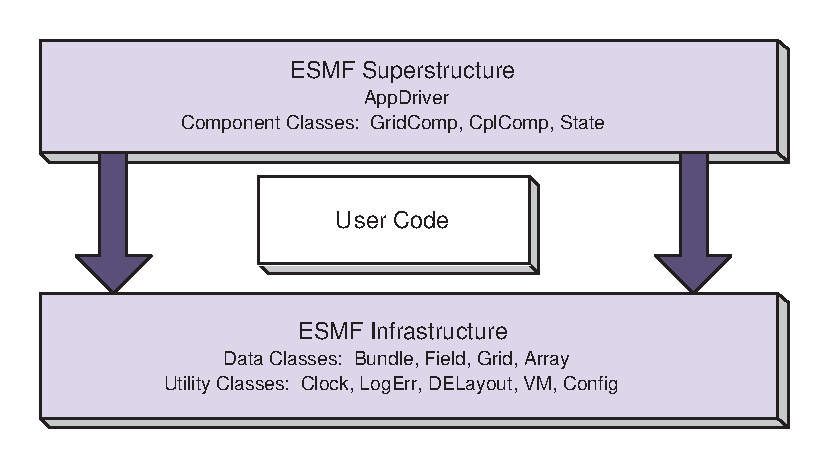
\includegraphics{ESMF_sandwich}}
\end{figure}
\end{center}


